\documentclass[11pt,a4paper]{article}
\usepackage{graphicx}   % Zum Einbinden von Bildern
\usepackage{amsmath} % Für mathematische Symbole
\usepackage{array}   % Für bessere Tabellenformatierung
\usepackage{booktabs} % Für schönere Tabellenlinien
\usepackage[table,xcdraw]{xcolor} % Für Farben
\usepackage{circuitikz}
\usepackage{graphicx}
\usepackage{graphicx}   % Zum Einbinden von Bildern
\usepackage[T1]{fontenc}


% Package imports und weitere Definitionen sind in einer seperaten Datei names preamble definiert.

%%%%%%%%%%%%%%%%%%%%%%%%%%%%%%%%%
% PACKAGE IMPORTS
%%%%%%%%%%%%%%%%%%%%%%%%%%%%%%%%%

\usepackage[utf8]{inputenc} % Zeichenkodierung
\usepackage[T1]{fontenc}    % Bessere Zeichenunterstützung
\usepackage[german]{babel}  % Korrekte deutsche Typografie
\usepackage[a4paper, left=2cm, right=2cm, top=2.5cm, bottom=2.5cm]{geometry}

\usepackage{graphicx}
\usepackage[export]{adjustbox}
\usepackage{microtype}
\usepackage{epstopdf}
\usepackage{float}
\usepackage{amsmath}
\usepackage{amssymb}
\usepackage{amstext}
\usepackage{amsfonts}
\usepackage{mathrsfs}
\usepackage{hyphenat}
\usepackage{fancyhdr}
\usepackage{qrcode}  % QR-Code generieren

\usepackage[most,many,breakable]{tcolorbox}

%%%%%%%%%%%%%%%%%%%%%%%%%%%%%%%%%%%%%%%%%%%%%%%%%%%%%%%%%%%%%%%%%%%%%%%%%%%%%%%%%%%%%%%%%%%%%%%%%%%%%%%%%%%%%%%%%%%%%%%%%%%%%%%%%%%%%%%%%%%%%
% Die folgende LaTeX preamble Datei basiert auf den Template von SeniorMars (https://github.com/SeniorMars/dotfiles/tree/main/latex_template)
%%%%%%%%%%%%%%%%%%%%%%%%%%%%%%%%%%%%%%%%%%%%%%%%%%%%%%%%%%%%%%%%%%%%%%%%%%%%%%%%%%%%%%%%%%%%%%%%%%%%%%%%%%%%%%%%%%%%%%%%%%%%%%%%%%%%%%%%%%%%%

%%%%%%%%%%%%%%%%%%%%%%%%%%%%%%
% FARBEN
%%%%%%%%%%%%%%%%%%%%%%%%%%%%%%

% Darf beliebig gewählt werden.

\definecolor{myg}{RGB}{56, 140, 70}
\definecolor{myb}{RGB}{45, 111, 177}
\definecolor{myr}{RGB}{199, 68, 64}
\definecolor{mytheorembg}{HTML}{F2F2F9}
\definecolor{mytheoremfr}{HTML}{00007B}
\definecolor{mylenmabg}{HTML}{FFFAF8}
\definecolor{mylenmafr}{HTML}{983b0f}
\definecolor{mypropbg}{HTML}{f2fbfc}
\definecolor{mypropfr}{HTML}{191971}
\definecolor{myexamplebg}{HTML}{F2FBF8}
\definecolor{myexamplefr}{HTML}{88D6D1}
\definecolor{myexampleti}{HTML}{2A7F7F}
\definecolor{mydefinitbg}{HTML}{E5E5FF}
\definecolor{mydefinitfr}{HTML}{3F3FA3}
\definecolor{notesgreen}{RGB}{0,162,0}
\definecolor{myp}{RGB}{197, 92, 212}
\definecolor{mygr}{HTML}{2C3338}
\definecolor{myred}{RGB}{127,0,0}
\definecolor{myyellow}{RGB}{169,121,69}
\definecolor{myexercisebg}{HTML}{F2FBF8}
\definecolor{myexercisefg}{HTML}{88D6D1}

%%%%%%%%%%%%%%%%%%%%%%%%%%%%
% TCOLORBOX SETUP
%%%%%%%%%%%%%%%%%%%%%%%%%%%%

\setlength{\parindent}{0cm} % Keine Indentierung nach einer Box

%%%%%%%%%%%%%%%%%%%%%%%%%%%%%%%%%%%%%%%%%%%%%%%%%%%%%%%%%%%%%%%%%%%%%%%%%%%%%%%%%%%%%%%%%%%%%%%%%%%%%%%%%%%%%%%%
% Es folgen ein paar "Kästen" die verwendet werden können für Definitionen, Beispielen, Aufgaben, etc.
% Falls einer nicht verwendet wird, einfach auskommentieren.
%%%%%%%%%%%%%%%%%%%%%%%%%%%%%%%%%%%%%%%%%%%%%%%%%%%%%%%%%%%%%%%%%%%%%%%%%%%%%%%%%%%%%%%%%%%%%%%%%%%%%%%%%%%%%%%%

%================================
% THEORIE BOX
%================================

\tcbuselibrary{theorems,skins,hooks}
\newtcbtheorem[number within=section]{Theorem}{Theorie}
{%
	enhanced,
	breakable,
	colback = mytheorembg,
	frame hidden,
	boxrule = 0sp,
	borderline west = {2pt}{0pt}{mytheoremfr},
	sharp corners,
	detach title,
	before upper = \tcbtitle\par\smallskip,
	coltitle = mytheoremfr,
	fonttitle = \bfseries\sffamily,
	description font = \mdseries,
	separator sign none,
	segmentation style={solid, mytheoremfr},
}
{th}

\tcbuselibrary{theorems,skins,hooks}
\newtcbtheorem[number within=section]{theorem}{Theorie}
{%
	enhanced,
	breakable,
	colback = mytheorembg,
	frame hidden,
	boxrule = 0sp,
	borderline west = {2pt}{0pt}{mytheoremfr},
	sharp corners,
	detach title,
	before upper = \tcbtitle\par\smallskip,
	coltitle = mytheoremfr,
	fonttitle = \bfseries\sffamily,
	description font = \mdseries,
	separator sign none,
	segmentation style={solid, mytheoremfr},
}
{th}


\tcbuselibrary{theorems,skins,hooks}

%================================
% Korollar
%================================

\tcbuselibrary{theorems,skins,hooks}
\newtcbtheorem[number within=section]{Corollary}{Korollar}
{%
	enhanced
	,breakable
	,colback = myp!10
	,frame hidden
	,boxrule = 0sp
	,borderline west = {2pt}{0pt}{myp!85!black}
	,sharp corners
	,detach title
	,before upper = \tcbtitle\par\smallskip
	,coltitle = myp!85!black
	,fonttitle = \bfseries\sffamily
	,description font = \mdseries
	,separator sign none
	,segmentation style={solid, myp!85!black}
}
{th}
\tcbuselibrary{theorems,skins,hooks}
\newtcbtheorem[number within=section]{corollary}{Korollar}
{%
	enhanced
	,breakable
	,colback = myp!10
	,frame hidden
	,boxrule = 0sp
	,borderline west = {2pt}{0pt}{myp!85!black}
	,sharp corners
	,detach title
	,before upper = \tcbtitle\par\smallskip
	,coltitle = myp!85!black
	,fonttitle = \bfseries\sffamily
	,description font = \mdseries
	,separator sign none
	,segmentation style={solid, myp!85!black}
}
{th}


%================================
% LENMA
%================================

\tcbuselibrary{theorems,skins,hooks}
\newtcbtheorem[number within=section]{Lenma}{Lenma}
{%
	enhanced,
	breakable,
	colback = mylenmabg,
	frame hidden,
	boxrule = 0sp,
	borderline west = {2pt}{0pt}{mylenmafr},
	sharp corners,
	detach title,
	before upper = \tcbtitle\par\smallskip,
	coltitle = mylenmafr,
	fonttitle = \bfseries\sffamily,
	description font = \mdseries,
	separator sign none,
	segmentation style={solid, mylenmafr},
}
{th}

\tcbuselibrary{theorems,skins,hooks}
\newtcbtheorem[number within=section]{lenma}{Lenma}
{%
	enhanced,
	breakable,
	colback = mylenmabg,
	frame hidden,
	boxrule = 0sp,
	borderline west = {2pt}{0pt}{mylenmafr},
	sharp corners,
	detach title,
	before upper = \tcbtitle\par\smallskip,
	coltitle = mylenmafr,
	fonttitle = \bfseries\sffamily,
	description font = \mdseries,
	separator sign none,
	segmentation style={solid, mylenmafr},
}
{th}


%================================
% VORSCHLAG
%================================

\tcbuselibrary{theorems,skins,hooks}
\newtcbtheorem[number within=section]{Prop}{Vorschlag}
{%
	enhanced,
	breakable,
	colback = mypropbg,
	frame hidden,
	boxrule = 0sp,
	borderline west = {2pt}{0pt}{mypropfr},
	sharp corners,
	detach title,
	before upper = \tcbtitle\par\smallskip,
	coltitle = mypropfr,
	fonttitle = \bfseries\sffamily,
	description font = \mdseries,
	separator sign none,
	segmentation style={solid, mypropfr},
}
{th}

\tcbuselibrary{theorems,skins,hooks}
\newtcbtheorem[number within=section]{prop}{Vorschlag}
{%
	enhanced,
	breakable,
	colback = mypropbg,
	frame hidden,
	boxrule = 0sp,
	borderline west = {2pt}{0pt}{mypropfr},
	sharp corners,
	detach title,
	before upper = \tcbtitle\par\smallskip,
	coltitle = mypropfr,
	fonttitle = \bfseries\sffamily,
	description font = \mdseries,
	separator sign none,
	segmentation style={solid, mypropfr},
}
{th}


%================================
% BEHAUPTUNG
%================================

\tcbuselibrary{theorems,skins,hooks}
\newtcbtheorem[number within=section]{claim}{Behauptung}
{%
	enhanced
	,breakable
	,colback = myg!10
	,frame hidden
	,boxrule = 0sp
	,borderline west = {2pt}{0pt}{myg}
	,sharp corners
	,detach title
	,before upper = \tcbtitle\par\smallskip
	,coltitle = myg!85!black
	,fonttitle = \bfseries\sffamily
	,description font = \mdseries
	,separator sign none
	,segmentation style={solid, myg!85!black}
}
{th}



%================================
% AUFGABE
%================================

\tcbuselibrary{theorems,skins,hooks}
\newtcbtheorem[number within=section]{Exercise}{Aufgabe}
{%
	enhanced,
	breakable,
	colback = myexercisebg,
	frame hidden,
	boxrule = 0sp,
	borderline west = {2pt}{0pt}{myexercisefg},
	sharp corners,
	detach title,
	before upper = \tcbtitle\par\smallskip,
	coltitle = myexercisefg,
	fonttitle = \bfseries\sffamily,
	description font = \mdseries,
	separator sign none,
	segmentation style={solid, myexercisefg},
}
{th}

\tcbuselibrary{theorems,skins,hooks}
\newtcbtheorem[number within=section]{exercise}{Aufgabe}
{%
	enhanced,
	breakable,
	colback = myexercisebg,
	frame hidden,
	boxrule = 0sp,
	borderline west = {2pt}{0pt}{myexercisefg},
	sharp corners,
	detach title,
	before upper = \tcbtitle\par\smallskip,
	coltitle = myexercisefg,
	fonttitle = \bfseries\sffamily,
	description font = \mdseries,
	separator sign none,
	segmentation style={solid, myexercisefg},
}
{th}

%================================
% BEISPIEL
%================================

\newtcbtheorem[number within=section]{Example}{Beispiel}
{%
	colback = myexamplebg
	,breakable
	,colframe = myexamplefr
	,coltitle = myexampleti
	,boxrule = 1pt
	,sharp corners
	,detach title
	,before upper=\tcbtitle\par\smallskip
	,fonttitle = \bfseries
	,description font = \mdseries
	,separator sign none
	,description delimiters parenthesis
}
{ex}

\newtcbtheorem[number within=section]{example}{Beispiel}
{%
	colback = myexamplebg
	,breakable
	,colframe = myexamplefr
	,coltitle = myexampleti
	,boxrule = 1pt
	,sharp corners
	,detach title
	,before upper=\tcbtitle\par\smallskip
	,fonttitle = \bfseries
	,description font = \mdseries
	,separator sign none
	,description delimiters parenthesis
}
{ex}

%================================
% DEFINITION
%================================

\newtcbtheorem[number within=section]{Definition}{Definition}{enhanced,
	before skip=2mm,after skip=2mm, colback=red!5,colframe=red!80!black,boxrule=0.5mm,
	attach boxed title to top left={xshift=1cm,yshift*=1mm-\tcboxedtitleheight}, varwidth boxed title*=-3cm,
	boxed title style={frame code={
					\path[fill=tcbcolback]
					([yshift=-1mm,xshift=-1mm]frame.north west)
					arc[start angle=0,end angle=180,radius=1mm]
					([yshift=-1mm,xshift=1mm]frame.north east)
					arc[start angle=180,end angle=0,radius=1mm];
					\path[left color=tcbcolback!60!black,right color=tcbcolback!60!black,
						middle color=tcbcolback!80!black]
					([xshift=-2mm]frame.north west) -- ([xshift=2mm]frame.north east)
					[rounded corners=1mm]-- ([xshift=1mm,yshift=-1mm]frame.north east)
					-- (frame.south east) -- (frame.south west)
					-- ([xshift=-1mm,yshift=-1mm]frame.north west)
					[sharp corners]-- cycle;
				},interior engine=empty,
		},
	fonttitle=\bfseries,
	title={#2},#1}{def}
\newtcbtheorem[number within=section]{definition}{Definition}{enhanced,
	before skip=2mm,after skip=2mm, colback=red!5,colframe=red!80!black,boxrule=0.5mm,
	attach boxed title to top left={xshift=1cm,yshift*=1mm-\tcboxedtitleheight}, varwidth boxed title*=-3cm,
	boxed title style={frame code={
					\path[fill=tcbcolback]
					([yshift=-1mm,xshift=-1mm]frame.north west)
					arc[start angle=0,end angle=180,radius=1mm]
					([yshift=-1mm,xshift=1mm]frame.north east)
					arc[start angle=180,end angle=0,radius=1mm];
					\path[left color=tcbcolback!60!black,right color=tcbcolback!60!black,
						middle color=tcbcolback!80!black]
					([xshift=-2mm]frame.north west) -- ([xshift=2mm]frame.north east)
					[rounded corners=1mm]-- ([xshift=1mm,yshift=-1mm]frame.north east)
					-- (frame.south east) -- (frame.south west)
					-- ([xshift=-1mm,yshift=-1mm]frame.north west)
					[sharp corners]-- cycle;
				},interior engine=empty,
		},
	fonttitle=\bfseries,
	title={#2},#1}{def}



%================================
% Lösung
%================================

\makeatletter
\newtcbtheorem{solution}{Lösung}{enhanced,
	breakable,
	colback=white,
	colframe=myb!80!black,
	attach boxed title to top left={yshift*=-\tcboxedtitleheight},
	fonttitle=\bfseries,
	title={#2},
	boxed title size=title,
	boxed title style={%
			sharp corners,
			rounded corners=northwest,
			colback=tcbcolframe,
			boxrule=0pt,
		},
	underlay boxed title={%
			\path[fill=tcbcolframe] (title.south west)--(title.south east)
			to[out=0, in=180] ([xshift=5mm]title.east)--
			(title.center-|frame.east)
			[rounded corners=\kvtcb@arc] |-
			(frame.north) -| cycle;
		},
	#1
}{def}
\makeatother

%================================
% FRAGE
%================================

\makeatletter
\newtcbtheorem{qstion}{Frage}{enhanced,
	breakable,
	colback=white,
	colframe=mygr,
	attach boxed title to top left={yshift*=-\tcboxedtitleheight},
	fonttitle=\bfseries,
	title={#2},
	boxed title size=title,
	boxed title style={%
			sharp corners,
			rounded corners=northwest,
			colback=tcbcolframe,
			boxrule=0pt,
		},
	underlay boxed title={%
			\path[fill=tcbcolframe] (title.south west)--(title.south east)
			to[out=0, in=180] ([xshift=5mm]title.east)--
			(title.center-|frame.east)
			[rounded corners=\kvtcb@arc] |-
			(frame.north) -| cycle;
		},
	#1
}{def}
\makeatother

%================================
% BEMERKUNG
%================================

\usetikzlibrary{arrows,calc,shadows.blur}
\tcbuselibrary{skins}
\newtcolorbox{note}[1][]{%
	enhanced jigsaw,
	colback=gray!20!white,%
	colframe=gray!80!black,
	size=small,
	boxrule=1pt,
	title=\textbf{Bemerkung:-},
	halign title=flush center,
	coltitle=black,
	breakable,
	drop shadow=black!50!white,
	attach boxed title to top left={xshift=1cm,yshift=-\tcboxedtitleheight/2,yshifttext=-\tcboxedtitleheight/2},
	minipage boxed title=2.5cm,
	boxed title style={%
			colback=white,
			size=fbox,
			boxrule=1pt,
			boxsep=2pt,
			underlay={%
					\coordinate (dotA) at ($(interior.west) + (-0.5pt,0)$);
					\coordinate (dotB) at ($(interior.east) + (0.5pt,0)$);
					\begin{scope}
						\clip (interior.north west) rectangle ([xshift=3ex]interior.east);
						\filldraw [white, blur shadow={shadow opacity=60, shadow yshift=-.75ex}, rounded corners=2pt] (interior.north west) rectangle (interior.south east);
					\end{scope}
					\begin{scope}[gray!80!black]
						\fill (dotA) circle (2pt);
						\fill (dotB) circle (2pt);
					\end{scope}
				},
		},
	#1,
}

%%%%%%%%%%%%%%%%%%%%%%%%%%%%%%%%%%%%%%%%%%%%%%%%%%%%%%%%%%%%%%%%%%
% Definierte Commands um in der template Datei zu verwenden.
%%%%%%%%%%%%%%%%%%%%%%%%%%%%%%%%%%%%%%%%%%%%%%%%%%%%%%%%%%%%%%%%%%

\newcommand{\thm}[2]{\begin{Theorem}{#1}{}#2\end{Theorem}}
\newcommand{\cor}[2]{\begin{Corollary}{#1}{}#2\end{Corollary}}
\newcommand{\mlenma}[2]{\begin{Lenma}{#1}{}#2\end{Lenma}}
\newcommand{\mprop}[2]{\begin{Prop}{#1}{}#2\end{Prop}}
\newcommand{\clm}[3]{\begin{claim}{#1}{}#2\end{claim}}
\newcommand{\exa}[2]{\begin{Example}{#1}{}#2\end{Example}}
\newcommand{\exe}[2]{\begin{Exercise}{#1}{}#2\end{Exercise}}
\newcommand{\dfn}[2]{\begin{Definition}[colbacktitle=red!75!black]{#1}{}#2\end{Definition}}
\newcommand{\sol}[2]{\begin{solution}{#1}{}#2\end{solution}}
\newcommand{\nt}[1]{\begin{note}#1\end{note}}

%%%%%%%%%%%%%%%%%%%%%%%%%%%%%%%%%%%%%%%%%%%
% INHALTSVERZEICHNIS
%%%%%%%%%%%%%%%%%%%%%%%%%%%%%%%%%%%%%%%%%%%


\usepackage{tikz}
\definecolor{doc}{RGB}{0,60,110}
\usepackage{titletoc}
\contentsmargin{0cm}
\titlecontents{section}[3.7pc]
{\addvspace{30pt}%
	\begin{tikzpicture}[remember picture, overlay]%
		\draw[fill=doc!60,draw=doc!60] (-7,-.1) rectangle (-0.1,.5);%
		\pgftext[left,x=-3.5cm,y=0.2cm]{\color{white}\Large\sc\bfseries Abschnitt\ \thecontentslabel};%
	\end{tikzpicture}\color{doc!60}\large\sc\bfseries}%
{}
{}
{\;\titlerule\;\large\sc\bfseries Seite \thecontentspage
	\begin{tikzpicture}[remember picture, overlay]
		\draw[fill=doc!60,draw=doc!60] (2pt,0) rectangle (4,0.1pt);
	\end{tikzpicture}}%
\titlecontents{subsection}[3.7pc]
{\addvspace{2pt}}
{\contentslabel[\thecontentslabel]{2pc}}
{}
{\hfill\small \thecontentspage}
[]
\titlecontents*{subsubsection}[3.7pc]
{\addvspace{-1pt}\small}
{}
{}
{\ --- \small\thecontentspage}
[ \textbullet\ ][]

\makeatletter
\renewcommand{\tableofcontents}{%
	\section*{%
	  \vspace*{-20\p@}%
	  \begin{tikzpicture}[remember picture, overlay]%
		  \pgftext[right,x=15cm,y=0.2cm]{\color{doc!60}\Huge\sc\bfseries \contentsname};%
		  \draw[fill=doc!60,draw=doc!60] (13,-.75) rectangle (20,1);%
		  \clip (13,-.75) rectangle (20,1);
		  \pgftext[right,x=15cm,y=0.2cm]{\color{white}\Huge\sc\bfseries \contentsname};%
	  \end{tikzpicture}}%
	\@starttoc{toc}}
\makeatother


% Variabeln definieren. Weitere Variabeln natürlich möglich

\def \autor{Rares Sahleanu}
\def \uebung{Übung 2}

\title{}
\date{}  % Kein Datum auf Standard-Titel

\begin{document}

% === DECKBLATT ===
\begin{titlepage}
	\centering
	{\Huge Netzwerke und Schaltungen II}\\[0.8cm]
	{\Large D-ITET}\\[0.8cm]
	{\Large FS2025}\\[3.5cm]

	{\Huge \textbf{\uebung}}\\[1cm]
	{\Large 28.2.2025}\\[3.5cm]

	\qrcode[height=6cm]{https://n.ethz.ch/~rsahleanu/}

	\vfill
	{\Large \textbf{\autor}}
\end{titlepage}

\newpage

% === AKTIVIERT KOPF- UND FUSSZEILEN AB SEITE 3 ===
\newpage
\pagestyle{fancy}

% Kopfzeile: Links - Mitte - Rechts (subtil & kleiner)
\fancyhead[L]{\small \textit{Netzwerke und Schaltungen II}}
\fancyhead[C]{\small \textit{\uebung}}
\fancyhead[R]{\small \textit{\autor}}

% Fußzeile: Seitenzahl in der Mitte
\fancyfoot[L]{}
\fancyfoot[C]{\thepage}
\fancyfoot[R]{}

% Linie in der Kopfzeile aktivieren, Fußzeile ohne Linie
\renewcommand{\headrulewidth}{0.4pt}
\renewcommand{\footrulewidth}{0pt}

%report === START DES DOKUMENTS ===

\section{Übersicht}  
Heute machen wir den großen Sprung von den zunächst sehr abstrakten Zeigern zur komplexen Wechselstromrechnung. Wir werden sehen, dass wir dank der Zeiger nicht mehr integrieren oder differenzieren müssen, um mit Kondensatoren und Induktivitäten zu arbeiten. Stattdessen können wir ihnen einfach einen komplexen Widerstand zuweisen. \\

Die zweite wichtige Erkenntnis wird sein, dass wir feststellen können, dass wir Stromteiler, Spannungsteiler, Kirchhoffsche Regeln und alles andere auch mit Zeigern verwenden können. \\

Damit hätten wir das Fundament für den Kurs gelegt, und wir können uns ab der nächsten Übungsstunde den wichtigen Themen widmen. Jeder, der es bisher sehr schwer fand, den kann ich beruhigen: Das „komplizierte neue Konzept“ des Kurses haben wir jetzt hinter uns, und ab jetzt nutzen wir nur noch bekannte Werkzeuge und Konzepte. :))

\newpage


\section{Komplexe Widerstände}
\vfill

Wir können reaktiven Bauteilen komplexe Widerstände (\textbf{Impedanz}) zuweisen. 
Die lineare Strom-Spannungs-Beziehung gilt damit auch mit \textbf{Zeigern}!

\begin{center}
\scalebox{1}{
\begin{tabular}{c c}
    \textbf{Bauteil} & \textbf{Impedanz} \\[8pt]
    Induktivität & $j \omega L$ \\
    Kapazität & $\frac{1}{j \omega C}$ \\
    Widerstand & $R$ \\
\end{tabular}
}
\end{center}
\vfill

\thm{Ohmsches Gesetz}{
    Das Ohmsche Gesetz gilt nun auch für \textbf{Zeiger}. 
    Wir verwenden jetzt jedoch statt des \textbf{Widerstands} die \textbf{Impedanz}:
    \begin{center}
        $\hat{u} = Z \cdot \hat{i}$
    \end{center}
}
\vfill

Eigentlich ist das bereits die Haupterkenntnis des ersten Kapitels. Alles, was ab jetzt folgt, sind lediglich Konsequenzen bzw. Folgerungen der dieser Theorie. Als zentrale Beispiele dienen bestimmte Arten von Spannungsteilern (sog. Filter), die nur spezifische Ausführungen normaler Spannungsteiler darstellen.
\vfill

\nt{
    Für ein tieferes Verständnis:  
    Eine \textbf{Impedanz} ist klar definiert durch ihren \textbf{Betrag} (Scheinwiderstand) und ihre \textbf{Phase} (Winkel in der komplexen Ebene).  
    Der \textbf{Betrag} gibt an, wie groß der \textbf{Widerstand} ist, unabhängig vom \textbf{imaginären Anteil}.  
    Die \textbf{Phase} beschreibt, wie stark der \textbf{Strom} bei angelegter \textbf{Spannung verzögert} wird.\footnote{Dafür habe ich ein Video vorbereitet.}
}
\vfill

\thm{Kirchhoff, Stromteiler, Spannungsteiler}{
    Alle bekannten Werkzeuge zur Berechnung von \textbf{Netzwerken} gelten weiterhin, nun jedoch mit \textbf{komplexen Widerständen}:
    \begin{center}
        \[
        \sum_{\text{Masche}} \hat{u} = 0 \quad \sum_{\text{Knoten}} \hat{i} = 0
        \]
    \end{center}

    Zusätzlich gelten auch die \textbf{Teilerregeln}:

    \begin{center}
        \textbf{Spannungsteilerregel:}
        \[
        \hat{u}_2 = \hat{u}_\text{ges} \cdot \frac{Z_2}{Z_1 + Z_2}
        \]
        
        \textbf{Stromteilerregel:}
        \[
        \hat{i}_2 = \hat{i}_\text{ges} \cdot \frac{Z_1}{Z_1 + Z_2}
        \]
    \end{center}
}
\newpage
\vfill
\nt{

\textbf{Tipp:} Wenn Ihr eine Formel bestimmt habt mit der ihr aber nicht ganz sicher seid, dann ist hier ein Tipp wie man das schnell ueberpruefen kann:
\begin{enumerate}
    \item Erinnert euch zuruck wie sich Induktivitaeten und Kapaziteten bei Gleichstrom und sehr hohen Frequenzen und Gleichspannung verhalten
    \item Stellt euch vor wie sich das Netzwerken in den beiden Oberen fallen verhalten wurde
    \item setzt in die Formel, die ihr errechnet habt, $\omega = 0$ und $\omega = \infty$ ein.
    \item interpretiert das Ergebnis
\end{enumerate}

}
\vfill
\section{Was wird wie genannt?}
Damit wir später alle dieselben Begriffe verwenden, ist es notwendig, eine Definition zu treffen. Diese ist, Gott sei Dank, sehr intuitiv und trägt jetzt nicht maßgeblich zum Verständnis bei.
\vfill
\dfn{Bezeichnungen}{
\begin{description}
  \item[Admittanz \(Y\)]  
    Kehrwert der Impedanz, gibt an, wie leicht Strom fließen kann: 
    \[
      Y=\frac{1}{Z}.
    \]
    
  \item[Impedanz \(Z\)]  
    Komplexer Widerstand in Wechselstromkreisen, definiert als:
    \[
      Z=R+jX.
    \]
    
  \item[Scheinwiderstand]  
    Betrag der Impedanz, der den ``effektiven`` Widerstand ohne Phasenbetrachtung angibt:
    \[
      |Z|=\sqrt{R^2+X^2}.
    \]
    
  \item[Phase]  
    Winkel \(\varphi\) zwischen Spannung und Strom, bestimmt durch:
    \[
      \varphi=\arctan\left(\frac{X}{R}\right).
    \]
    
  \item[Realteil \(R\)]  
    Der ohmsche Anteil der Impedanz, verantwortlich für den Energieverbrauch.
    
  \item[Imaginärteil \(X\)]  
    Der reaktive Anteil (Blindwiderstand), bedingt durch induktive oder kapazitive Elemente.
\end{description}
}

\exe{Aufgabe}{
	Bestimme die Phase und den Btrag dieser Impedanz: \\ \begin{center}
	    $\underline{Z} = R+j\omega L + \frac{1}{j\omega C}$
	\end{center}\\
    Tipp: $\frac{1}{j} = -j$
}
\newpage
\section{Graphische Tipps und Visualisierung}
\subsection{Visualisierung - Impedanz}
\begin{center}
    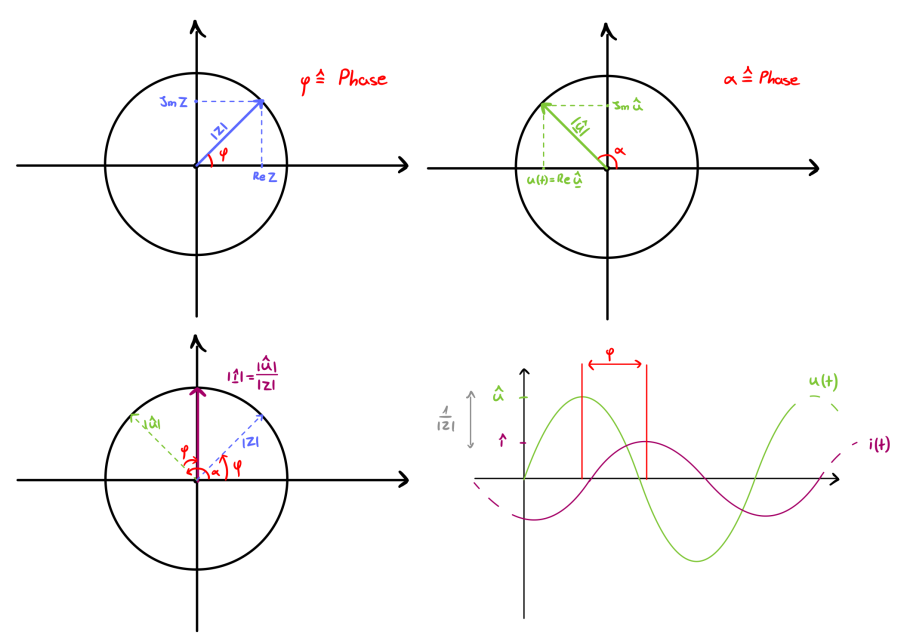
\includegraphics[width=0.9\textwidth]{last.png}

\end{center}
In diesem Beispiel wird ein einfaches Beispiel einer Impedanz an einer Spannungsquelle behandelt. die oberen Zwei bilder zeigen jeweils die Impedanz und die Spannung in Zeigerdarstellung. Unten ist dann der resultierende Strom in Zeit und Zeigerdarstellung. Hervorgehoben wurde die isolierte Auswirkng der Impedanz auf den Strom. Dieser ist um $\varphi = arg(Z)$ gegenueber der Spannung voreilend und ist gegenueber der Spannung um den Betrag $|\underline{Z}|$ skaliert\footnote{Eine Animierte Simulation auf meiner Website: https://n.ethz.ch/~rsahleanu/nus2/utils/impe.html}\\
\textbf{Beachte:} Im Falle enes Realen widerstands, sind Strom und Spannung in Phase, da $arg(Z) = 0$ ist
\subsection{Intuition - Wie koennen Spannung und Strom nicht in Phase sein? }



\noindent%
{
  \begin{minipage}[t]{0.4\textwidth}
    \vspace{0pt} % Erzwingt Top-Ausrichtung
    \centering
    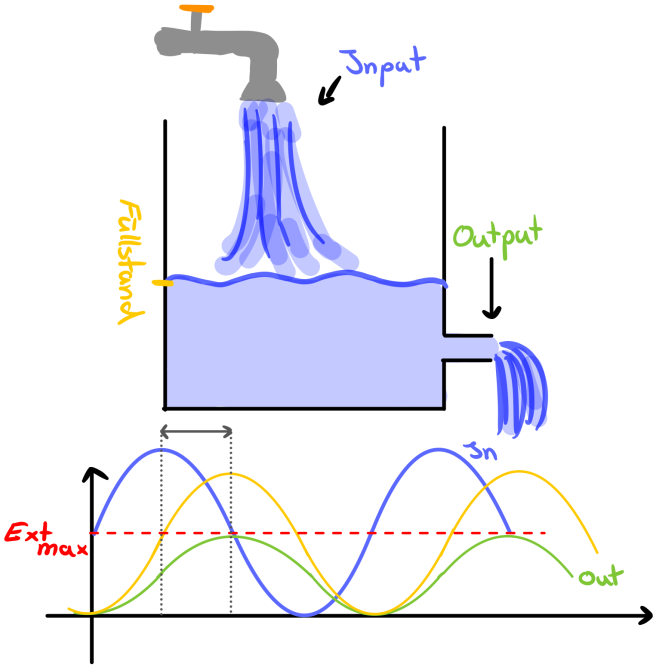
\includegraphics[width=\textwidth]{analogy.png}

  \end{minipage}%
}
\hfill%
{
  \begin{minipage}[t]{0.55\textwidth}
    \vspace{0pt} % Erzwingt Top-Ausrichtung
    
 Je höher der Wasserstand im Kanister, desto mehr Wasser fließt heraus, und Wasser kann nur maximal halb so schnell ausfließen, wie man eingießen kann. Wenn ich eine sinusförmige Menge Wasser eingieße, ist der Kanister erst nach Erreichen der maximalen Eingießgeschwindigkeit am vollsten und leert sich dementsprechend auch am schnellsten. Die Maxima der Gießgeschwindigkeit und der Wasseraustrittsgeschwindigkeit bzw. des Wasserstands sind demnach nicht in Phase.
  \end{minipage}%
}



\newpage
\section{Grundlagen der Netzwerkanalyse}
Die Netzwerkanalyse beschäftigt sich mit der Berechnung von Strömen und Spannungen in elektrischen Netzwerken. Wichtige Konzepte sind:

\subsection{Kirchhoffsche Gesetze}
Die Kirchhoffsche Regeln werden zur Analyse von elektrischen Netzwerken verwendet.

\thm{Theorie}{
	Das ist eine Theorie Box
}

\dfn{Definition}{
	Definitionen sind gut fürs Verständnis.
}


\cor{Korollar}{
	Wow! Ein Korollar!
}

\subsection{Maschen- und Knotenanalyse}
Die Maschen- und Knotenanalyse ist eine wichtige Methode zur Netzwerkanalyse.

\mlenma{Lenma}{
	Braucht man Lenmas wirklich?
}

\mprop{Vorschlag}{
	Ein Vorschlag ist immer gut!
}

\nt{
	NUS ist cool!
}


\subsection{Zweipoltheorie}
Ein elektrisches Zweipolnetz kann als Thevenin- oder Norton-Ersatzschaltung modelliert werden.

\clm{}{
	Die Erde ist flach!
}

\exa{Beispiel}{
	Beispiele sind immer gut.
}

\subsection{Zusatzaufgaben}
\begin{itemize}
	\item Aufgabe 1: Berechnen Sie die Spannungen in einem einfachen Widerstandsnetzwerk mit zwei Maschen.
	\item Aufgabe 2: Verwenden Sie die Knotenpunktanalyse, um die Ströme in einem Netzwerk mit drei Widerständen und einer Spannungsquelle zu bestimmen.
\end{itemize}

\exe{Aufgabe}{
	Diese Aufgabe ist in einer Box.
}

\vspace{1cm}
% === ZWEITES KAPITEL ===
\section{Frequenzgang und Filter}
Der Frequenzgang eines Netzwerks beschreibt die Abhängigkeit der Übertragungsfunktion von der Frequenz.

\sol{Lösung}{
	Das ist die Lösung zur Aufgabe
}

\subsection{Tiefpass- und Hochpassfilter}
Tiefpass- und Hochpassfilter ermöglichen die Frequenzselektion.

\subsection{Bandpass- und Bandsperrfilter}
Bandpass- und Bandsperrfilter entfernen spezifische Frequenzbereiche.

\subsection{Bode-Diagramme}
Bode-Diagramme stellen den Frequenzgang von Systemen grafisch dar.

\subsection{Zusatzaufgaben}
\begin{itemize}
	\item Aufgabe 1: Bestimmen Sie die Grenzfrequenz eines einfachen RC-Tiefpassfilters.
	\item Aufgabe 2: Zeichnen Sie das Bode-Diagramm eines gegebenen RLC-Bandpassfilters.
\end{itemize}

\end{document}
